\documentclass [border=12pt] {standalone}
\usepackage{tikz}

\begin{document}
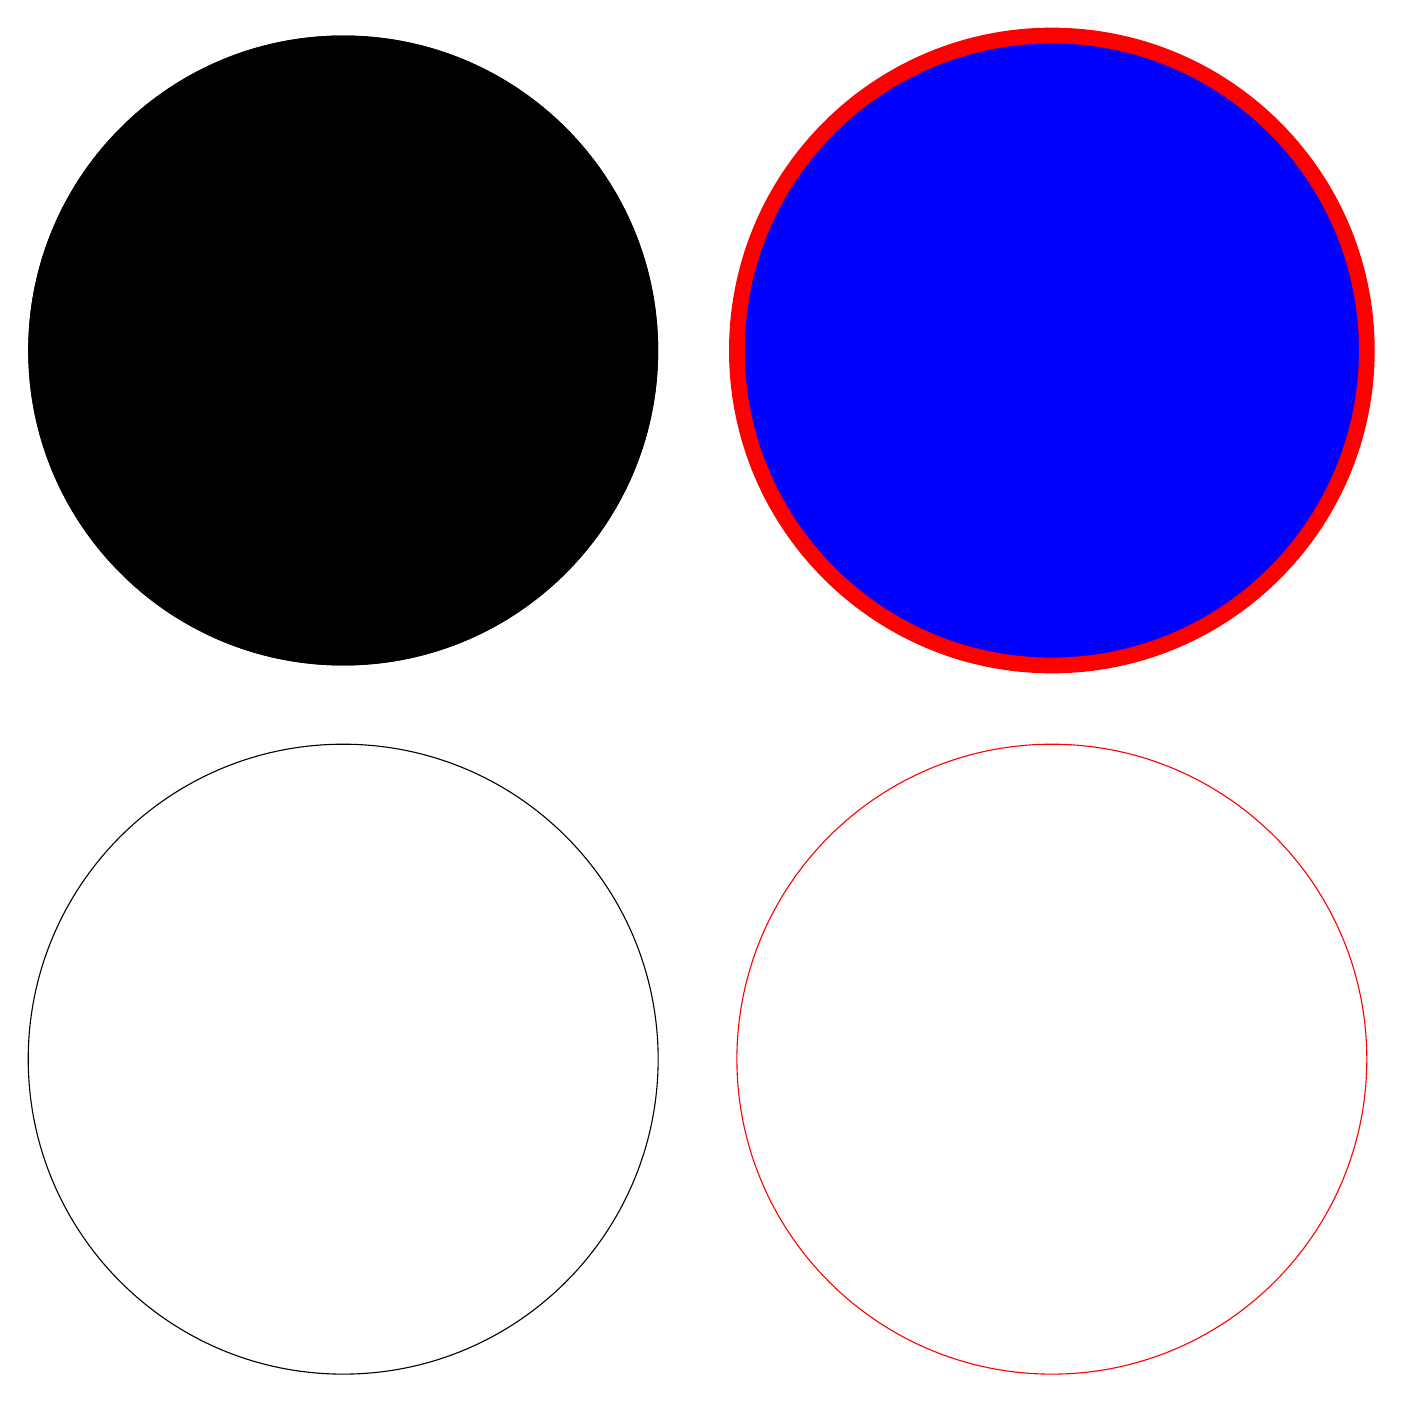
\begin{tikzpicture}

% 画空心圆
\draw (0,0) circle(4);
\draw [red] (9,0) circle[radius=4cm]; % radius:半径
% 画实心圆
\fill (0,9) circle(4);
% 画实心圆
\fill (0,9) circle(4);
% 画带边框的实心圆
\filldraw [draw=red, fill=blue, line width=0.2cm] (9,9) circle(4);

\end{tikzpicture}
\end{document}
